\mcchap{Manuale utente}{cap:manuale}

\section{Requisiti software}
Il progetto è stato realizzato utilizzando \emph{ambiente di sviluppo integrato} (IDE) Pycharm Community.
Per l'esecuzione della dashboard sono richieste le seguenti dipendenze.
\begin{itemize}
 \item Python 3.8.5
 \item Pandas
 \item Plotly 
 \item Dash 
 \item Dash Bootstrap Components
 \end{itemize}
 
 \section{Installazione dipendenze}
 Per installare le librerie richieste è sufficiente lanciare i seguenti comandi dal termianle integrato in Pycharm.
 
 \begin{itemize}
     \item \texttt{\$ pip install pandas}
     \item \texttt{\$ pip install plotly==4.12.0}
     \item \texttt{\$ pip install dash==1.17.0}
     \item \texttt{\$ pip install dash-bootstrap-components}
 \end{itemize}
 
 \begin{figure}[htp]
    \centering
    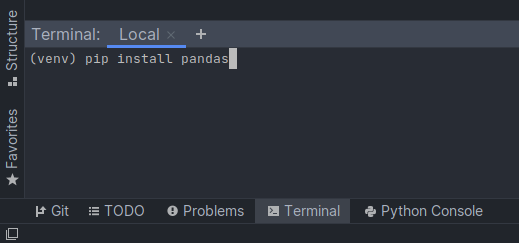
\includegraphics[width=10cm]{pycharm_terminal}
    \caption{Terminale integrato in Pycharm}
    \label{fig:pycharm_termianl}
\end{figure}

\section{Esecuzione}
 
 
